	Praca nad niewidoczną dla użytkownika końcowego częścią generycznych modułów zaowocowała opracowaniem 3 niezależnych modułów. To czym jest generyczny moduł, najłatwiej opisać na przykładzie jednej z metody programowania - programowania uogólnionego. Koncepcja ta oparta jest o założenie, że wiele fragmentów kodu jest niepotrzebnie powtarzanych tylko dlatego, że służą do przetwarzania różnych danych w identyczny sposób. Podejście generyczne pozwala na tworzenie ogólnych algorytmów, gdzie wymagania dotyczące danych, są nieokreślone lub zdefiniowane na poziomie abstrakcyjnych typów danych. 

\subsection{Strony obiektów domenowych oraz tabele}
	Podczas analizy wymagań warstwy biznesowej aplikacji demonstracyjnej stało się jasne, że podejście do reprezentacji danych w formie tabel, czy też wyświetlenia informacji o pojedynczym obiekcie domenowym, nie będzie operacją trywialną. Kluczowe było wybranie efektywnego sposobu reprezentacji obiektu lub obiektów domenowych w wybranym formacie. Z uwagi na przyjęte wymaganie funkcjonalne oraz w myśl zasady \textbf{DRY} (\ref{concept:dry}), tworzenie kolejnych klas z kodem odpowiedzialnym za powstawanie struktury tabeli lub strony internetowej było niedopuszczalne. Nie udało się również znaleźć żadnej biblioteki wspierającej taką funkcjonalność. Strony obiektów domenowych, zwane dalej \textbf{info page}, oraz tabele, to moduły generyczne ponieważ:
	\begin{itemize}
		\item algorytm pobierania danych jest niezależny od danych na poziomie typów danych, tj. możliwe było jego zaimplementowanie w abstrakcyjnej klasie generycznej, nie posiadającej na etapie kompilacji żadnej informacji o konkretnym typie obiektów, jakie klasa będzie przetwarzać,
		\item algorytm zdefiniowany jest raz,
		\item algorytm jest elastyczny,
		\item komponenty są w stanie samodzielnie skonwertować dane do typu prostego (liczba, wartość logiczna lub łańcuch znakowy), który można bezproblemowo zaprezentować po stronie klienta,
		\item finalne implementacje odpowiedzialne są jedynie za:
		\begin{itemize}
			\item dostarczenie informacji o budowie komponentu,
			\item dostarczenie wartości dla atrybutów dynamicznych, nie związanych z typem przetwarzanych danych
		\end{itemize}		 
	\end{itemize}
	
	Artefaktem definiującym powyższe założenie, będącym korzeniem całej hierarchii klas tych komponentów, jest interfejs \textbf{ComponentBuilder} (listening \ref{app:component_builder}). To właśnie ten interfejs jest następnie używany w kontrolerach odpowiedzialnych za mapowanie żądań pobrania definicji lub danych z poszczególnych komponentów. Same kontrolery nie zależą bezpośrednio od konkretnych implementacji, ale opierają się na \textbf{API} wspólnym dla wszystkich obiektów typu \textbf{ComponentBuilder}. Szczególnie ważne są tutaj następujące metody:
	\begin{itemize}
		\item \textbf{getDefinition()} - zadaniem tej metody jest zwrócenie struktury, definicji danego komponentu,
		\item \textbf{getData()} - zadaniem tej metody jest zwrócenie danych danego komponentu.
	\end{itemize}
	
	\begin{code}
		\inputminted[
			linenos=true,
			firstline=32,
			lastline=46,
			fontfamily=monospace,
			obeytabs=true,
			samepage=true,
			fontsize=\scriptsize
		]{java}{\SpringatomScrPath{/web/component/builders/ComponentBuilder.java}}
		\caption[\textbf{ComponentBuilder - korzeń hierarchii modułu komponentów}]{
			\textbf{ComponentBuilder} - korzeń hierarchii modułu komponentów, który opisuje rolę tego rodzaju obiektów w systemie, źródło: opracowanie własne				
		}
		\label{app:component_builder}
	\end{code}
	
	\paragraph{Problem wielu zapytań AJAX} \hspace{0pt} \\
	Aplikacja internetowa korzysta z zapytań do serwera aby pobierać treść, dane oraz zasoby, które mogą zostać zaprezentowane użytkownikowi. Z każdym zapytaniem wiążą się jednak koszty, których nie sposób jest uniknąć. Narzut związany z inicjacją zapytania, odpowiedzią serwera, jej wielkością oraz samym czasem odpowiedzi jest kwestią, którą należy uwzględnić. Problemem, który pojawił się podczas projektowania algorytmu renderowania \textbf{info page} oraz tabeli wynikał z uogólnionej koncepcji według, której miały one działać. Niemniej, bez wiedzy o typie obiektu domenowego, którego atrybuty miały być przedstawione na stronie lub którego obiekty miały być wyświetlone w tabeli, nie było możliwości wstępnego przygotowania struktury takiego komponentu. Jedną z możliwości rozwiązania tego problemu było wykonanie dwóch oddzielnych zapytań do serwera, najpierw po definicję, a następnie po dane. Inną ewentualnością było wystosowanie pojedynczego zapytania, gdzie odpowiedź miałaby zawierać informacja o charakterystyce i danych. W drugim przypadku kwestią dyskusyjną stawał się rozmiar odpowiedzi, a także format w jakim przedstawiona musiałaby być definicja, aby możliwe było jej efektywne przetworzenie na odpowiednią strukturę DOM.  
	
	Wyjściem z sytuacji było skorzystanie z możliwości dynamicznego definiowania zawartości stron HTML, budowanych poprzez pliki JSP. Idea zakładała wykorzystanie mechanizmów dostępnych tylko i wyłącznie po stronie serwera, takich jak \textbf{tagi JSTL} i serwisy aplikacji, do utworzenia struktury DOM i odesłania gotowego dokumentu w odpowiedzi na żądania. Alternatywą byłoby budowanie kolejnych elementów strony przez \textbf{JavaScript}, co, nawet przy wykorzystaniu bibliotek takich jak \textbf{jQuery}, byłoby operacją mozolną i podatną na błędy. W kontekście omawianych komponentów, wybrane podejście zostało zastosowane zarówno dla stron obiektów domenowych, jak i tabel. Jedynie w przypadku \textbf{info page}, również dane, umieszczane są w strukturze dokumentu po stronie serwera. 
	
	\paragraph{Problem źródła danych} \hspace{0pt} \\
	Główna funkcjonalność tej części aplikacji demonstracyjnej sprowadza się do wydajnej i rozszerzalnej zmiany reprezentacji pewnej informacji na inną. Nie byłoby to możliwe bez źródła danych. Problemem z repozytorium, które byłoby w stanie sprostać zadaniu pobrania obiektów konkretnego typu, sprowadzał się właśnie do typu. W myśl idei jaka przyświeca programowaniu uogólnionemu, to nie dane są ważne, ale algorytm ich przetwarzania. Niemniej, dzięki wsparciu biblioteki \textbf{Spring Data JPA} (\ref{tech:spring_data_jpa}), kwestia ta została łatwo rozwiązania. Wspomniane repozytoria, w kontekście \textbf{Spring Data JPA}, są niczym innym jak generycznymi interfejsami. Wykorzystując ten fakt oraz własność typów generycznych języka Java, gdzie typ uogólniony, znajdujący się w deklaracji klasy, może zostać użyty w polach oraz metodach tej klasy (listining \ref{app:generic_types_matching}), repozytoria zdefiniowane zostały jako pola poszczególnych komponentów. Ostatecznie, korzystając z funkcjonalność szkieletu aplikacji \textbf{Spring}, pozwalając na wstrzykiwania zależności generycznych klas. Zachowane zostało bezpieczeństwo typów, a generyczne algorytmy uzyskały możliwość korzystania ze źródła danych.
	\begin{code}
		\inputminted[
			linenos=true,
			firstline=69,
			lastline=76,
			fontfamily=monospace,
			obeytabs=true,
			samepage=false,
			fontsize=\scriptsize
		]{java}{\SpringatomScrPath{/web/component/builders/table/TableComponentBuilder.java}}
		\caption[Typy generyczne w deklaracji oraz polach klasy w języku Java]{
			Typy generyczne w deklaracji oraz polach klasy w języku Java, źródło: opracowanie własne	
		}
		\label{app:generic_types_matching}
	\end{code}
	\paragraph{Problem identyfikacji \textbf{ComponentBuilder}} \hspace{0pt} \\
	Komponenty zostały tak zaprojektowane, aby zminimalizować poziom zależności między konkretnymi instancjami \textbf{ComponentBuilder} oraz odpowiadającym im elementów interfejsu użytkownika. Problematyczne okazało się zdefiniowanie powiązania pozwalającego nawigować między oboma artefaktami. Rozwiązanie oparte zostało na adnotacjach języka Java oraz zdolności szkieletu aplikacji \textbf{Spring} do wybierania obiektów opatrzonych konkretnymi adnotacjami spośród wszystkich zdefiniowanych.  
	\begin{code}
		\inputminted[
			linenos=true,
			firstline=40,
			lastline=53,
			fontfamily=monospace,
			obeytabs=true,
			samepage=false,
			fontsize=\scriptsize
		]{java}{\SpringatomScrPath{/web/component/builders/annotation/ComponentBuilds.java}}
		\caption[\textbf{ComponentBuilds} - adnotacja opisująca \textbf{omponentBuilder}]{
			\textbf{ComponentBuilds} - adnotacja opisująca \textbf{ComponentBuilder}, źródło: opracowanie własne
		}
		\label{app:componentBuilds_annotation}
	\end{code}	
	
	\textbf{ComponentBuilds} pozwala na zdefiniowanie następujących informacji:
	\begin{itemize}
		\item unikatowy klucz pod którym obiekt istnieje w aplikacji,
		\item typ budowanego komponentu: strona lub tabela
	\end{itemize}
	Dzięki \textbf{EntityBased} dany komponent zostaje ściśle powiązany z pewną klasą biznesowego modelu danych, jako artefakt zdolny utworzyć reprezentację obiektu lub obiektów tej klasy. Wszystkie te informacje pozwalają na pobranie obiektu \textbf{ComponentBuilder} skonkretyzowanego na przygotowanie tabeli, której kolejne wiersze odpowiadają konkretnym obiektom domenowym lub gotowego na utworzenie definicji strony domenowej.  
	\begin{code}
		\inputminted[
			linenos=true,
			firstline=27,
			lastline=33,
			fontfamily=monospace,
			obeytabs=true,
			samepage=false,
			fontsize=\scriptsize
		]{java}{\SpringatomScrPath{/web/component/builders/annotation/EntityBased.java}}
		\caption[\textbf{EntityBased} - adnotacja opisująca klasę obiektu domenowego, z którą związana jest konkretny \textbf{ComponentBuilder}]{
			\textbf{EntityBased} - adnotacja opisująca klasę obiektu domenowego, z którą związana jest konkretny \textbf{ComponentBuilder}, źródło: opracowanie własne
		}
		\label{app:entityBased_annotation}
	\end{code}	

\subsection{InfoPage - strony obiektów modelu danych}
	\textbf{InfoPage} jest komponentem budującym reprezentację obiektu domenowego jako strony internetowej. Składają się na niego artefakty opisujące strukturę strony, skonkretyzowana, pod kątem przetwarzania danych, implementacja interfejsu \textbf{ComponentBuilder} (\ref{app:component_builder}), klasy pomocnicze, usprawniające proces budowania struktury i pozyskiwania definicji komponentów na podstawie unikatowego klucza, klasy obiektu domenowego związanej z daną stroną lub adresu wpisanego w oknie przeglądarki. 
	
	\paragraph{Definicja komponentu InfoPage} \hspace{0pt} \\
	Pełna definicja \textbf{InfoPage} składa się z dwóch elementów: rozszerzenia klasy \textbf{EntityInfoPageComponentBuilder} i \textbf{SEntityInfoPage}. \textbf{SEntityInfoPage} (listining \ref{app:sEntityInfoPage}) dostarcza metadanych o:
	\begin{itemize}
		\item klasie obiektu domenowego,
		\item unikatowym identyfikatorze strony,
		\item unikatowym kluczu będącym częścią adresu danej strony
	\end{itemize}
	Podczas startu, aplikacja pobiera konkretne implementacje \textbf{SEntityInfoPage}, które istnieją w programie jako obiekty, dzięki wsparciu szkieletu aplikacji \textbf{Spring}, który automatycznie tworzy instancje opatrzonych odpowiednią adnotacją (\textbf{Component}, \textbf{Service} lub \textbf{Repository}). Dzięki temu procesowi możliwe jest odwoływanie się do meta obiektu \textbf{InfoPage} poprzez dowolny atrybut opisujący go. 
	\clearpage
	\begin{code}
			\inputminted[
				linenos=true,
				firstline=25,
				lastline=32,
				fontfamily=monospace,
				obeytabs=true,
				samepage=false,
				fontsize=\scriptsize
			]{java}{\SpringatomScrPath{/web/infopages/SEntityInfoPage.java}}
			\caption[\textbf{SEntityInfoPage} - interfejs opisujący metadane związane ze stroną domenową]{
				\textbf{SEntityInfoPage} - interfejs opisujący metadane związane ze stroną domenową, źródło: opracowanie własne
			}
			\label{app:sEntityInfoPage}
	\end{code}	
	
	\paragraph{Algorytm pobrania danych dla strony domenowej} \hspace{0pt} \\
	\textbf{EntityInfoPageComponentBuilder} jest implementacją \textbf{ComponentBuilder} (\ref{app:component_builder}) zawierającą skonkretyzowany algorytm pobierania wartości atrybutów, będących częścią danej strony. Jego zadaniem jest również przetworzenie danych na reprezentacją, którą będzie można wyświetlić po stronie klienta, jako prosty łańcuch znakowy lub liczbę. Widoczna w interfejsie \textbf{ComponentBuilder} metoda \textbf{getDefinition} pozostaje na tym poziomie nie zaimplementowana. Przyczyna tego leży w odmienności poszczególnych stron obiektów domenowych, sprowadzającej się do różnej ich struktury, różnych atrybutów, które będą widoczne i ostatecznie do innej klasy biznesowego modelu danych, skojarzonej z komponentem \textbf{InfoPage}.
	
	\subparagraph{Rozwiązanie problemu reprezentacji danych} \hspace{0pt} \\
	W przypadku strony domenowej atrybutami, które wymagały rozwiązania niespójności typów danych, były relacje klucz obcy - klucz główny. Sytuacja kiedy obiekt, będący podmiotem danej strony, zależy od innego obiektu, została rozwiązania jako przedstawienie takiej zależności w postaci hiperłącza do strony domenowej, jeśli takowa została zdefiniowana (innymi słowy, jeśli w systemie można było znaleźć definicję klasy \textbf{SEntityInfoPage} oraz odpowiadającej jej implementacji \textbf{EntityInfoPageComponentBuilder}. Odwrotna sytuacja miała miejsce, kiedy podmiot strony był zależnością dla innych obiektów domenowych. Rozwiązana została ona poprzez przekazanie, jako wartości dla atrybutu, informacji niezbędnych do załadowania tabeli. Analogicznie do pierwszego przypadku, również w tym momencie, koniecznie było najpierw ustalenie, czy w aplikacji istnieje odpowiednia implementacja klasy \textbf{TableComponentBuilder}.
	Problem nieczytelnej wartości typów wyliczeniowych został rozwiązany z wykorzystaniem specjalnego pliku, zawierającego listę wszystkich wartości wszystkich typów wyliczeniowych wraz z ich czytelną wartością. 
	 
	\begin{code}
			\inputminted[
				linenos=true,
				firstline=98,
				lastline=149,
				fontfamily=monospace,
				obeytabs=true,
				samepage=false,
				fontsize=\scriptsize
			]{java}{\SpringatomScrPath{/web/infopages/component/builder/EntityInfoPageComponentBuilder.java}}
			\caption[\textbf{EntityInfoPageComponentBuilder} - implementacja pozyskania danych dla strony obiekty domenowego]{
				\textbf{EntityInfoPageComponentBuilder} - implementacja pozyskania danych dla strony obiekty domenowego, źródło: opracowanie własne
			}
			\label{app:entityInfoPageComponentBuilder}
	\end{code}	
	
	Utworzenie nowej strony sprowadza się sprowadza się do zaimplementowania \textbf{EntityInfoPageComponentBuilder}, oznaczenia nowej klasy adnotacjami: \textbf{ComponentBuilds} (listing \ref{app:componentBuilds_annotation}) i \textbf{EntityBased} (listing \ref{app:entityBased_annotation}) oraz utworzenia nowej implementacji interfejsu \textbf{SEntityInfoPage}. 
	\clearpage
	\paragraph{Proces renderowania strony domenowej} \hspace{0pt} \\
	\begin{figure}[H]
		\centering
		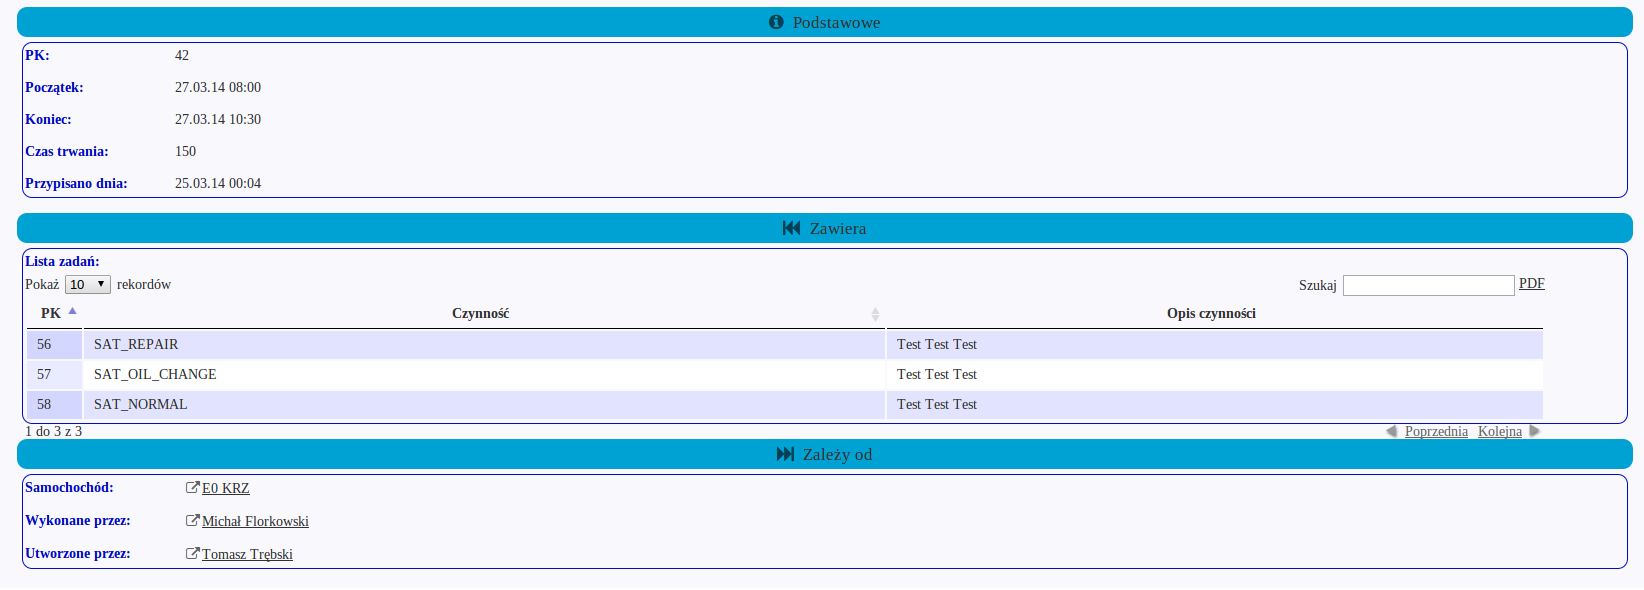
\includegraphics[width=1.0\textwidth]{images/infoPage}
		\caption[Strona domenowa dla spotkania]{
			Strona domenowa dla spotkania, źródło: opracowanie własne	
		}
		\label{app:infoPage}
	\end{figure}
	
	Na rysunku \ref{app:infoPage} pokazana została strona domenowa obiektu opisującego pojedyncza wizytę w warsztacie samochodowym. Zdefiniowane zostały 3 panele z atrybutami. Panel podstawowy oraz dwa panele opisujące relacje zachodzące między spotkaniem a innymi obiektami. Spotkanie posiada więc listę zadań oraz zostało przypisane do pewnego samochodu, zgłoszone i wykonane przez konkretnych mechaników. Listing kodu \ref{app:infoPageSrcCode} przedstawia fragmentu kodu Java odpowiedzialny za zbudowania struktury strony.
	\begin{code}
		\inputminted[
			linenos=true,
			firstline=50,
			lastline=75,
			fontfamily=monospace,
			obeytabs=true,
			samepage=false,
			fontsize=\scriptsize
		]{java}{\SpringatomScrPath{/webmvc/pages/builders/AppointmentInfoPageComponentBuilder.java}}
		\caption[Strona domenowa dla spotkania - kod źródłowy]{Strona domenowa dla spotkania - kod źródłowy, źródło: opracowanie własne}
		\label{app:infoPageSrcCode}
	\end{code}
	
	Proces, w wyniku którego wywołana została metoda z listingu \ref{app:infoPageSrcCode}, tworząca strukturę strony, oraz wywołujący metodą pokazaną na listingu \ref{app:entityInfoPageComponentBuilder}}, która zwraca dane dla konkretnych atrybutów, ilustruje poniższa tabela:
	\begin{center}
		\begin{longtable}{| p{2.5cm} | p{13cm} |}
			\caption[Proces renderowania strony domenowej]{Proces renderowania strony domenowej}\tabularnewline	
			
			% header
			\hline
				\multicolumn{1}{|c|}{\textbf{Krok}} 		&
				\multicolumn{1}{|c|}{\textbf{Opis}} 		\tabularnewline
			\hline
			\endfirsthead
			
			\multicolumn{2}{c}
			{{\bfseries \tablename\ \thetable{} -- kontynuacja...}} \tabularnewline
			\hline
				\multicolumn{1}{|c|}{\textbf{Krok}} 		&
				\multicolumn{1}{|c|}{\textbf{Opis}} 		\tabularnewline
			\hline
			\endhead
				
			\hline
				\multicolumn{2}{|r|}{{Następna strona...}} \tabularnewline
			\hline
			\endfoot
	
			\hline
			\endlastfoot	
			% end of header
			
			% body starts her
			\textbf{1}							&
			Zdarzeniem inicjującym proces renderowania strony domenowej jest wpisanie w przeglądarce adresu, 
			który zostaje rozpoznany przez aplikację jako wskazujący na komponent \textbf{InfoPage}. Jest to możliwe ponieważ 
			adres komponentu posiadana określony format: \textbf{/ip/\{klucz strony\}/\{klucz główny\}/\{wersja\}}. Najważniejszym elementem
			adresu jest \textbf{klucz strony} (listining \ref{app:sEntityInfoPage}). 
			\tabularnewline
			\hline
			\textbf{2}							&
			Żądanie zostaje zmapowane do metody \textbf{getInfoPageView} (listining \ref{app:svInfoPageController}). Jej zadaniem jest
			pobranie meta danych strony domenowej na podstawie unikatowego klucza strony, wspomnianego w punkcie 1. Obiekt klasy \textbf{SInfoPage}
			zostaje umieszczony w odpowiedzi razem z hiperłączem, pod którym dostępny będzie dokument HTML zawierający gotową stronę \textbf{InfoPage}.
			\tabularnewline
			\hline
			\textbf{3}							&
			Po stronie klienta, kod JavaScript zajmuje się przygotowaniem asynchronicznego żądania po gotowy widok strony, dostępny pod adresem
			z punktu 2.
			\tabularnewline
			\hline
			\textbf{4}							&
			Żądanie, wysłane z punkcie 3, zostaje zmapowane do metody \textbf{getInfoPageViewData} (listining \ref{app:svInfoPageController}). Metoda pobiera instancję
			klasy \textbf{ComponentBuilder}, która spełnia następujące wymagania:
			\begin{itemize}
				\item buduje strukturę strony domenowej,
				\item związana jest z typem obiektu domenowego
			\end{itemize}
			Znaleziony \textbf{ComponentBuilder} jest następnie umieszczany w odpowiedzi razem z widokiem, będącym szablonem (listing \ref{app:domain_render_jsp}) przyszłej strony.
			Szablon zaprojektowany został dla jednoczesnego tworzenia dokumentu HTML, zawierającego atrybuty oraz odpowiadające im wartości. 
			To właśnie z poziomu pliku JSP, w przypadku stron obiektów domenowych, wywoływane są metody 
			interfejsu \textbf{ComponentBuilder} pozwalające na pobranie jej struktury oraz danych. 
		\end{longtable}
	\end{center}
	
	\begin{code}
		\inputminted[
			linenos=true,
			firstnumbe=59,
			firstline=59,
			lastline=95,
			fontfamily=monospace,
			obeytabs=false,
			samepage=false,
			fontsize=\scriptsize
		]{java}{\SpringatomScrPath{/webmvc/controllers/SVInfoPageController.java}}
		\caption[SVInfoPageController - kontroler obsługujący żądania komponentu \textbf{InfoPage}]{SVInfoPageController - kontroler obsługujący żądania komponentu \textbf{InfoPage}}
		\label{app:svInfoPageController}
	\end{code}

	\begin{code}
		\inputminted[
			gobble=5,
			linenos=true,
			firstnumbe=64,
			firstline=64,
			lastline=91,
			fontfamily=monospace,
			obeytabs=false,
			samepage=false,
			fontsize=\scriptsize
		]{jsp}{../SpringAtom_thesis/src/main/webapp/ui/ip/_render.jsp}
		\caption[Szablon strony obiektu domenowego]{Fragment szablonu strony obiektu domenowego, tworzący ciało tabeli}
		\label{app:domain_render_jsp}
	\end{code}
	
\subsection{TableBuilder}
	Rzadko zdarza się żeby aplikacja nie wymagała korzystania z tabel do prezentowania danych. Są one szczególnie użyteczne zwłaszcza w momencie, kiedy ilość możliwych obiektów do jednorazowego wyświetlenia sięga co najmniej kilkudziesięciu elementów. Każda z nich opisana jest zarówno przez zbiór danych, jak i przez zbiór kolumn. Aby poprawnie zdefiniować tabelę wymagane jest podanie obu zbiorów. Istnieją dwie całkowicie odmienne koncepcje tego zagadnienia: statyczna oraz dynamiczna. W przypadku podejścia statycznego, struktura tabeli jest ręcznie umieszczana w strukturze DOM dokumentu HTML. Takie podejście sprawia jednak, że tabela jest stała, zarówno pod kątem tego co wyświetla, jak również w jaki sposób to robi, każda modyfikacja zbioru danych, wymaga więc ręcznej aktualizacji. Dynamiczną realizację tej kwestii można podzielić na przypadki, gdzie:
	\begin{enumerate}
		\item struktura jest statyczna, źródło danych jest dynamiczne,
		\item struktura oraz dane są dynamiczne
	\end{enumerate}
	
	\paragraph{Problem reprezentacji danych} \hspace{0pt} \\
	Problematyczne w obu podejściach nie okazuje się jednak ani wprowadzenie schematu mapującego poszczególne kolumny na odpowiadające im pola danych, ani też automatyzacja procesu wpisującego poprawną, w rozumieniu języka HTML, definicję tabeli do struktury DOM dokumentu. W przypadku pliku JSP rozwiązanie wymagałoby by ustalenia zbioru kolumn, pobrania danych z repozytorium, ręcznego wpisania statycznych elementów tabeli, takich jak na przykład nagłówek i utworzenia ciała tabeli (kolejnych wierszy) na podstawie zbioru danych. Inne podejście zakładałoby wykorzystanie biblioteki JavaScript dostarczającej dodatkowej warstwy abstrakcji nad procesem definiowania tabeli oraz zdolnej do wygenerowania zapytania Ajax pod wskazany adres, pod którym dostępny byłby zbiór danych. Problemem jest reprezentacja danych. Poniższe zestawienie opisuje wybrane przypadki, gdzie pokazane zostały potencjalne rozwiązania, a rzeczywista i oczekiwana reprezentacja danych jest od siebie różna:
	
	\begin{center}
		\begin{longtable}{| p{4cm} | p{12cm} |}
			\caption[Zestawienie problemów reprezentacji danych dla tabel]{
				Zestawienie problemów reprezentacji danych dla tabel	
				\label{app:tablesProblems}
			}\tabularnewline	
			
			% header
			\hline
				\multicolumn{1}{|c|}{\textbf{Problem}} 						&
				\multicolumn{1}{|c|}{\textbf{Potencjalne rozwiązanie}} 		\tabularnewline
			\hline
			\endfirsthead
			
			\multicolumn{2}{c}
			{{\bfseries \tablename\ \thetable{} -- kontynuacja...}} \tabularnewline
			\hline
				\multicolumn{1}{|c|}{\textbf{Problem}} 						&
				\multicolumn{1}{|c|}{\textbf{Potencjalne rozwiązanie}} 		\tabularnewline
			\hline
			\endhead
				
			\hline
				\multicolumn{2}{|r|}{{Następna strona...}} \tabularnewline
			\hline
			\endfoot
	
			\hline
			\endlastfoot	
			% end of header
			
			% body starts her
			\textbf{Relacja klucz główny - klucz obcy}							&
			Wykonanie następnego zapytania do repozytorium danych, pobranie powiązanego obiektu. Kolejną
			niewiadomą w tym przypadku jest niestety to, jaki atrybut powiązanego obiektu wybrać, który
			jednoznacznie by go opisywał, a w pierwszej kolejności wiedza, które z atrybutów należy
			interpretować jako relacje. 
			\tabularnewline
			\hline
			\textbf{Data jako znacznik czasowy}								&
			Przechowanie daty jako znaczników czasowych jest zalecane, ponieważ jest to rozwiązanie przenośne,
			pozwalające na uniknięcie problemu operowania na datach jako łańcuchach znakowych, w których format
			zapisu jest kwestią zależną od programisty i podatną na błędy. Utworzenie zrozumiałej reprezentacji
			wymagałoby by wiedzy o tym, które kolumny krotki bazy danych, to tak naprawdę daty.
			\tabularnewline
			\hline
			\textbf{Typy wyliczeniowe}											&
			\textbf{Typ wyliczeniowy}, w kontekście języka Java, to specjalny rodzaj klasy, pozwalający na tworzenie
			stałych w trakcie kompilacji programu, które, w sposób niezmienny, opisują pewną właściwość obiektu, z 
			którą są związane. Na poziomie bazy danych możliwe jest przechowanie wartości typu wyliczeniowego jako
			łańcucha znakowego. Problemem jest tutaj format w jakim kolejne pozycje typu wyliczeniowego są definiowane.
			Najczęściej pisane dużymi literami, nie posiadając spacji nie są dobrym kandydatem do bezpośredniego
			zaprezentowania w tabeli. Ponownie, rozwiązanie tego problemu, wymagałoby wiedzy nie tyle o tym, które
			z atrybutów należy interpretować jako pozycje typu wyliczeniowego, ale także tego, o który typ
			wyliczeniowy chodzi oraz danych, opisujących jego wartość w sposób zrozumiały dla użytkownika. 
		\end{longtable}
	\end{center}
	
	\paragraph{TableComponentBuilder} \hspace{0pt} \\
	\textbf{TableComponentBuilder} jest implementacją interfejsu \textbf{ComponentBuilder} (listing \ref{app:componentBuilds_annotation}), który został zaprojektowany do budowany definicji oraz zbioru danych dla tabel. Rozwiązuje on problemy zdefiniowane w tabeli \ref{app:tablesProblems} oraz dostarcza sposobu wsparcia następujących aspektów pracy z tabelami:
	\begin{itemize}
		\item wsparcie dla sortowania po stronie serwera,
		\item wsparcie dla filtrowania po stronie serwera,
		\item wsparcie dla dynamicznych kolumn, nie związanych bezpośrednio z typem obiektów, które tabela wyświetla
	\end{itemize}
	Działa on w oparciu o bibliotekę \textbf{Dandelion Datatables} (\ref{tech:dandelion}). Wykorzystanie biblioteki \textbf{Dandelion}, pozwoliło na ograniczenie ilości kodu niezbędnego do poprawnego wpisania definicji tabeli do struktury dokumentu HTML. Odpowiedzialność za ten proces została oddelegowana do wykorzystanej biblioteki, podobnie jak wykonanie asynchronicznego zapytania pod adres, pod którym znajduje się zbiór danych dla tabeli.
	
	\paragraph{Algorytm budowania zbioru danych} \hspace{0pt} \\
	Algorytm odpowiedzialny za utworzeniu zbioru danych jest podobny do tego, który zdefiniowano dla \textbf{InfoPage} (listing \ref{app:entityInfoPageComponentBuilder}). Różnice polegają na formacie w jakim dane są zwracane oraz w sposobie generowania zapytania do repozytorium danych. Podczas gdy strona domenowa była związana z pojedynczym obiektem, tabela związana jest z pewną ich liczbą. Dlatego też algorytm został skonkretyzowany na zwrócenia danych jako kolekcji, gdzie kolejne jej elementy odpowiadają kolejnym wierszom tabeli. Uwzględnia on także stronnicowanie, które polega na zwróceniu jedynie pewnego wycinka danych, zamiast wszystkich możliwych rekordów z bazy danych.
	\clearpage
	\begin{code}
		\inputminted[
			gobble=4,
			linenos=true,
			firstline=117,
			lastline=151,
			fontfamily=monospace,
			obeytabs=false,
			samepage=false,
			fontsize=\scriptsize
		]{java}{\SpringatomScrPath{/web/component/builders/table/TableComponentBuilder.java}}
		\caption[\textbf{TableComponentBuilder} - fragment implementacji pozyskania zbioru danych dla tabel]{\textbf{TableComponentBuilder} - fragment implementacji algorytmu pozyskania zbioru danych dla tabel}
		\label{app:tableComponentBuilder}
	\end{code}
	
	Warto w tym miejscu wspomnieć o podwójnym trybie działania algorytmu. W momencie, gdy tabela działa w kontekście komponentu \textbf{InfoPage}, nadrzędnym obiektem, zwanym dalej kontekstem, jest obiekt z którym skojarzona jest strona obiektu domenowego. Dla tego przypadku, tabela zwraca zbiór danych, który dla wspomnianego kontekstu jest wynikiem transformacji zależności klucz główny - klucz obcy. Z drugiej strony, komponent tabeli może zostać umieszczony na podstronie, gdzie kontekst nie jest zdefiniowany. W takim wypadku, budowany zbiór danych nie jest zawężany do żadnej relacji między poszczególnymi obiektami. Widoczne na listingu \ref{app:tableComponentBuilder} wywołanie metody \textbf{getPridacate} wykorzystuje funkcję \textbf{isInContext} (listing \ref{app:tcd_isInContext}), która rozpoznaje czy kontekst jest obecny i tym samym decyduje o zachowaniu tabeli. Jeśli kontekst istnieje tworzony jest predykat. Zadanie to realizowane jest na poziomie finalnych implementacji klas.
		
	\begin{code}
		\inputminted[
			gobble=1,
			linenos=true,
			firstline=290,
			lastline=293,
			fontfamily=monospace,
			obeytabs=false,
			samepage=false,
			fontsize=\scriptsize
		]{java}{\SpringatomScrPath{/web/component/builders/table/TableComponentBuilder.java}}
		\caption[\textbf{isInContext} - metoda \textbf{TableComponentBuilder} określająca tryb pracy]{
			\textbf{isInContext} - metoda \textbf{TableComponentBuilder} określająca tryb pracy komponentu dla algorytmu budowania zbioru danych, źródło: opracowanie własne
		}
		\label{app:tcd_isInContext}
	\end{code}
	
	\paragraph{Proces renderowania tabeli} \hspace{0pt} \\
	\begin{figure}[hb]
		\centering
		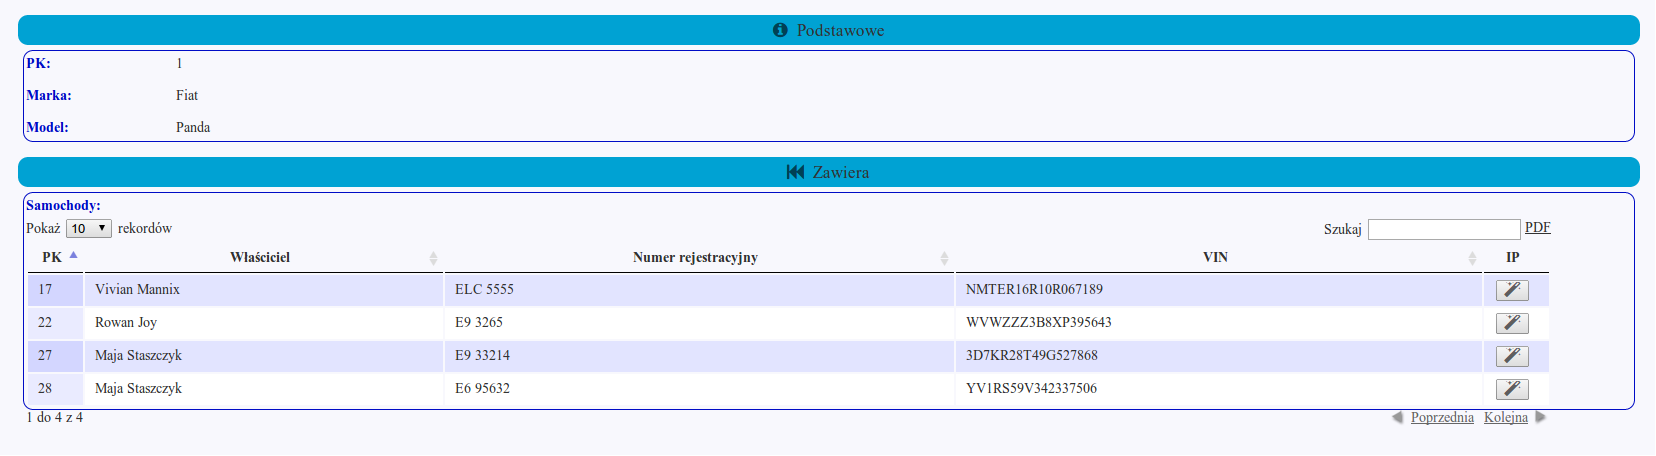
\includegraphics[width=1.0\textwidth]{images/table_inContext}
		\caption[Tabela wyświetlająca wszystkie pojazdy danej marki i modelu]{
			Tabela wyświetlająca wszystkie pojazdy danej samochodu \textbf{Fiat Panda}, źródło: opracowanie własne
		}
		\label{app:tableInContext}
	\end{figure}	
	
	Tabela na rysunku \ref{app:tableInContext} odpowiada implementacja klasy \textbf{TableComponentBuilder} widocznej na listingu \ref{app:cars_table_src_code}. Posiada ona 5 kolumn, z których 4 utworzone zostały w metodzie \textbf{buildDefinition} klasy \textbf{CarsTableBuilder}. Ostatnia kolumna dodawana jest domyślnie do każdej tabeli, jeśli dla obiektu, stanowiącego de facto źródło danych pojedynczego wiersza, istnieje definicja komponentu \textbf{InfoPage}. Wspomniana kolumna zawiera akcję, której wywołanie prowadzi do strony obiektu domenowego.

	\begin{code}
		\inputminted[
			linenos=true,
			firstline=35,
			lastline=77,
			fontfamily=monospace,
			obeytabs=true,
			samepage=false,
			fontsize=\scriptsize
		]{java}{\SpringatomScrPath{/webmvc/pages/builders/CarsTableBuilder.java}}
		\caption[Klasa definiująca strukturę tabeli wyświetlającej listę samochodów]{
			\emph{CarsTableBuilder} - klasa definiująca strukturę tabeli wyświetlającej listę samochodów, źródło: opracowanie własne	
		}
		\label{app:cars_table_src_code}
	\end{code}
	
	Proces, w wyniku którego tabela widoczna na rysunku \ref{app:tableInContext}, jest dostępna w interfejsie użytkownika, przedstawiony został w poniższej tabeli:
	\begin{center}
		\begin{longtable}{| p{1.5cm} | p{14cm} |}
			\caption[Proces renderowania tabeli]{Proces renderowania tabeli}\tabularnewline	
			
			% header
			\hline
				\multicolumn{1}{|c|}{\textbf{Krok}} 		&
				\multicolumn{1}{|c|}{\textbf{Opis}} 		\tabularnewline
			\hline
			\endfirsthead
			
			\multicolumn{2}{c}
			{{\bfseries \tablename\ \thetable{} -- kontynuacja...}} \tabularnewline
			\hline
				\multicolumn{1}{|c|}{\textbf{Krok}} 		&
				\multicolumn{1}{|c|}{\textbf{Opis}} 		\tabularnewline
			\hline
			\endhead
				
			\hline
				\multicolumn{2}{|r|}{{Następna strona...}} \tabularnewline
			\hline
			\endfoot
	
			\hline
			\endlastfoot	
			% end of header
			
			% body starts her
			\textbf{1}							&
			Tabela istnieje w kontekście strony domenowej. Zdefiniowany na 
			listingu \ref{app:domain_render_jsp} kod, obsługuje ten przypadek z wykorzystaniem
			technologii JavaScript. Po stronie klienta generowane jest 
			asynchroniczne zapytanie, które zostaje zmapowane na wywołanie metody \textbf{getTableBuilderPost} (listing \ref{app:svTableBuilderController})
			kontrolera \textbf{SVTableBuilderController}. Metoda odszukuje 
			instancję \textbf{TableComponentBuilder} na podstawie przekazanego w zapytaniu parametru \textbf{builderId},
			a następnie umieszcza odnaleziony obiekt w odpowiedzi razem z nazwą widoku.
			\tabularnewline
			\hline
			\textbf{2}							&
			Wybrany w punkcie 2 widok to plik JSP, w którym, z przekazanej instancji obiektu \textbf{ComponentBuilder}, pobierana jest
			definicja tabeli. Uzyskane informacje są, w dalszej części, ustawiane jako atrybuty tagu \textbf{JSP} z biblioteki \textbf{Dandelion Datables}.
			Od tego momentu, proces budowania struktury DOM nowej tabeli jest obsługiwany przez wybraną biblioteką. Warto tutaj zwrócić uwagę na atrybut \textbf{url},
			pod którym udostępnione będą dane dla tabeli. Adres tworzony jest na podstawie unikatowego identyfikatora obiektu \textbf{TableComponentBuilder}.
			\tabularnewline
			\hline
			\textbf{3}							&
			\textbf{Dandelion Datatables} po stworzeniu struktury tabeli 
			generuje asynchroniczne zapytanie pod podany w punkcie 2 adres. Żądanie
			zostaje zmapowane na wywołanie metody \textbf{getBuilderData} (listing \ref{app:svTableBuilderController}) 
			kontrolera \textbf{SVTableBuilderController}. Metoda pobiera instancję
			\textbf{ComponentBuilder} i wywołuje metodę \textbf{getData}. 
			Dane są następnie zwracane w postaci pliku \textbf{JSON} do tabeli po stronie klienta aplikacji.
		\end{longtable}
	\end{center}	
	
	\clearpage
	\begin{code}
		\inputminted[
			linenos=true,
			firstline=67,
			lastline=103,
			fontfamily=monospace,
			obeytabs=false,
			samepage=false,
			fontsize=\scriptsize
		]{java}{\SpringatomScrPath{/webmvc/controllers/SVTableBuilderController.java}}
		\caption[SVTableBuilderController - kontroler obsługujący żądania komponentu \textbf{TableBuilder}]{
			SVTableBuilderController - kontroler obsługujący żądania komponentu \textbf{TableBuilder}, źródło: opracowanie własne
		}
		\label{app:svTableBuilderController}
	\end{code}	
		
\subsection{RBuilder - szablony raportów biznesowych}
	\textbf{RBuilder} jest modułem aplikacji praktycznej, realizującym koncepcję tworzenia szablonów raportów biznesowych, będących opisem struktury gotowego raportu. Generowanie raportów zostało zrealizowane z wykorzystaniem biblioteki \textbf{Dynamic Jasper} (\ref{tech:jasperReports}). Istniejące narzędzia do tworzenia szablonów, zrozumiałych przez tę bibliotekę, nie istnieją jako aplikacje działające w środowisku przeglądarki internetowej. Głównym założeniem funkcjonalnym komponentu \textbf{RBuilder} jest więc dostarczenie logiki oraz widoku pozwalających na przygotowanie szablonu w oknie przeglądarki, a następnie wygenerowanie gotowego raportu jako dokumentu \textbf{PDF}, \textbf{XLS}, \textbf{HTML} lub \textbf{CSV}.
	
	\paragraph{Model danych - reprezentacja szablonu}   \hspace{0pt} \\
	Szablon raportu należy rozumieć jako obiekt domenowy \textbf{SReport} oraz klasę \textbf{ReportConfiguration}. Pierwszy z wymienionych obiektów zapisywany jest w bazie danych i pozwala na stwierdzenie gdzie zapisany został szablon oraz gdzie znajduje się zserializowany obiekt drugiej z wymienionych klas. \textbf{ReportConfiguration} dostarcza informacji trudnych do efektywnego zamodelowania na poziomie bazy danych. Są to informacje opisujące źródło danych:
	\begin{itemize}
		\item wybrane obiekty domenowe,
		\item wybrane atrybutu obiektów domenowych	
	\end{itemize}	 
	oraz strukturę nowego raportu, widoczną dla użytkownika:
	\begin{itemize}
		\item tytuł,
		\item podtytuł,
		\item kolumny,
		\item informacje o kolumnach grupujących, według których dane będą pogrupowane,
		\item wybrane reprezentacje, w których dane umieszczone w poszczególnych kolumnach, będą zaprezentowane w raporcie
	\end{itemize}
	
	\paragraph{Serwisy - przetwarzanie danych}  					\hspace{0pt} \\
		Serwisy komponentu \textbf{RBuilder} dostarczają metod, dzięki którym możliwe jest zapisanie szablonu, wygenerowanie z niego raportu 
	w wybranej przez użytkownika reprezentacji i dostarczenie danych do przewodnika tworzenia nowego raportu. Dostarczone usługi to:
	\begin{itemize}
		\item ustalenie możliwych formatów danego atrybuty, a tym samym kolumny w raporcie,
		\item tworzenie obiektu domenowego w zależności od konfiguracji raportu,
		\item generowanie raportu,
		\item zapis i odczyt informacji o raporcie z bazy danych oraz systemu plików.
	\end{itemize}
	Funkcjonalność tej grupy klas dla komponentu \textbf{RBuilder} można podzielić na następujące bloki:
	\begin{center}
		\begin{longtable}{| p{2.5cm} | p{13cm} |}
			\caption[Bloki funkcjonalne modelu serwisów \textbf{RBuilder}]{
				Bloki funkcjonalne modelu serwisów \textbf{RBuilder}			
			}
			\label{app:rbuilder_services_functionality_table}
			\tabularnewline	
			
			\hline
				\multicolumn{1}{|c|}{\textbf{Grupa}} &
				\multicolumn{1}{|c|}{\textbf{Funkcjonalność}} \tabularnewline
			\hline
			\endfirsthead
			
			\multicolumn{2}{c}
			{{\bfseries \tablename\ \thetable{} -- kontynuacja...}} \tabularnewline
			\hline
				\multicolumn{1}{|c|}{\textbf{Grupa}} &
				\multicolumn{1}{|c|}{\textbf{Funkcjonalność}} \tabularnewline
			\hline
			\endhead
				
			\hline
				\multicolumn{2}{|r|}{{Następna strona...}} \tabularnewline \hline
			\endfoot
			\hline
			\endlastfoot	
			
			\emph{Operation Management} 									& 
			Grupa \textbf{Operation Management} odpowiedzialna jest za tworzenie obiektu domenowego \textbf{SReport} w zależności
			od ilości tabel wybranych dla konkretnego raportu. Lista klas:
			\begin{itemize}
				\item SingleEntityRBuilderCreateOperation - obsługuje przypadek, w którym źródłem danych dla nowego raportu jest pojedyncza tabela w bazie danych,
				\item MultipleEntitiesRBuilderCreateOperation - obsługuje przypadek, w którym źródłem danych jest wiele tabel.
			\end{itemize}	
			\tabularnewline				
			\hline
			
			\emph{Data Management}											&
			Klasy z grupy \textbf{Data Management} zostały zaprojektowane do pobierania danych takich jak:
			\begin{itemize}
				\item informacje o typach obiektów domenowych, które można uwzględnić w raportach. Takie klasy adnotowane są 
				przez \emph{\@{}ReportableEntity}, a ich lista udostępniana jest poprzez interfejs \emph{ReportableEntityResolver},
				\item listę kolumn wraz z ich cechami takimi jak nazwa, typ danych przechowywanych w klasie, w odpowiadającej jej polu oraz możliwe ich reprezentacje. Informacje tego typu udostępniane są poprzez interfejs \emph{ReportableColumnResolver},
				\item listę powiązań między modelami w uproszczonej formie na potrzeby wybierania tabel podczas projektowania raportu. 
				Na obecną chwile możliwe jest utworzenie jedynie nieprzechodnich powiązań opisanych na bazowym poziomie przez relacje
				klucz główny - obcy. Dane tego typu udostępnione są przez interfejs \emph{ReportableAssociationResolver}. 
			\end{itemize}
			\hline
			
			\emph{Dynamic Jasper Operation}								&
			\emph{JasperBuilderService} jest jedyną klasą tej grupy, dostarczającą możliwości utworzenia skompilowanego
			szablonu do pliku \textbf{*.jasper}. Obecnie wspiera ona przypadek pojedynczej tabeli, jako źródła danych raportu. Jej zadaniem jest
			utworzenie obiektu klasy \textbf{DynamicReport} poprzez ustawienie, na tym obiekcie, następujących informacji:
			\begin{itemize}
				\item tytuł,
				\item podtytuł,
				\item opis,
				\item język,
				\item szerokość odpowiednich sekcji jak nagłówek, stopka itp.,
				\item lista kolumn,
				\item lista kolumn według których dane mają być grupowane.
			\end{itemize}
			\hline
			
			\emph{Generic helper}												&
			\emph{ReportBuilderService} jest artefaktem serwisu, przekazującym sterowanie do modułu
			\textbf{Operation Management}, celem utworzenia instancji obiektu domenowego \textbf{SReport} oraz wsparcia
			dla operacji renderowania raportu w konkretnej reprezentacji. Kiedy pierwsza z funkcji jest trywialna w kontekście złożoności, służąc
			jedynie separacji zadań i zmniejszeniu kohezji klas, druga z wymienionych metod jest dużo bardziej złożona.
			Jej celem jest pobranie danych wymaganych przez moduł \textbf{Spring}, używanych później do zrenderowania raportu 
			w wybranym przez użytkownika formacie, na przykład PDF. Operacje przez nią wykonywane to:
			\begin{itemize}
				\item pobranie obiektu domenowego z bazy danych dla danego numeru raportu, 
				\item deserializacja skompilowanego pliku \textit{*.jasper} z systemu plików,
				\item utworzenie źródła danych, zrozumiałego przez bibliotekę \textbf{DynamicJasper}, na podstawie informacji takich jak lista kolumn, ich typ, wybrany typ reprezentacji danych w kolumnie
			\end{itemize}
			\hline
		\end{longtable}
	\end{center}
				
	%%%%%%%%%%%%%%%%%%%%%%%%%%%%%%%%%%%%%%%%%%%%%%%%%%%%%%%%%%%%%%%%%%%%%%%%%%%%%%%%%%%%%%%%%%%%%%%%%%%%%%%%%%%%%%%%%%%%%%%%%%%%%%%%%%%%%%%%%%%%
	
	\paragraph{Warstwa widoku} 					\hspace{0pt} \\
	
	\begin{figure}[H]
		\centering
		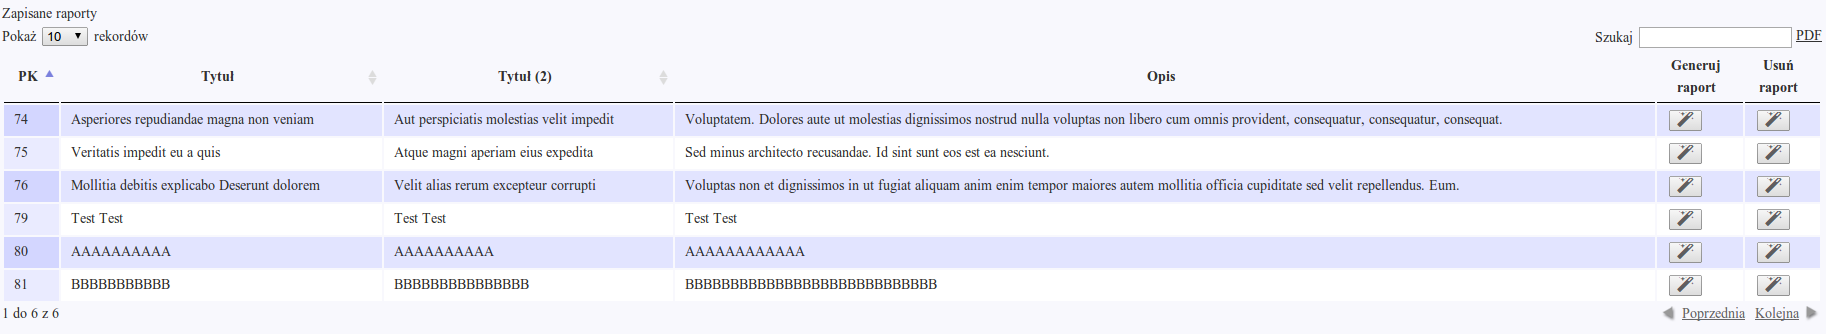
\includegraphics[width=1.0\textwidth]{images/rbuilder_table}
		\caption[Tabela wyświetlająca zapisane szablony]{
			Tabela wyświetlająca zapisane szablony, źródło: opracowanie własne
		}
		\label{app:wizard_savedReports}
	\end{figure}	
	
	Na część obsługującą widok komponentu \textbf{RBuilder} składają się:
	\begin{itemize}
		\item tabela z istniejącymi raportami,
		\item przewodnik tworzenia nowego raportu (opisany w rozdziale \textbf{ReportBuilder - tworzenie szablonów raportów biznesowych} \ref{wizard:rbuilder})
	\end{itemize}

	Tabela jest obiektem należącym do warstwy widoku, utworzonym z wykorzystaniem komponentu \textbf{TableBuilder} (\ref{app:tableComponentBuilder}). W tabeli
	widoczne są wszystkie zapisane w systemie szablony. Dodatkowo do każdego z wierszy przypisane zostały akcje pozwalające na:
	\begin{itemize}
		\item generowanie nowego raportu,
		\item usunięcie szablonu z bazy danych.
	\end{itemize}
	
	\begin{figure}[H]
		\centering
		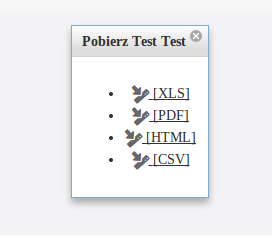
\includegraphics[width=0.5\textwidth]{images/rbuilder_generateReport}
		\caption[Generowanie nowego raportu - wybór docelowego formatu]{
			Generowanie nowego raportu - wybór docelowego formatu, źródło: opracowanie własne
		}
		\label{app:wizard_newReport_generateReport}
	\end{figure}
	
	Usunięcie jest prostą, z punktu widzenia użytkownika, operacją, ponieważ nie widzi on niczego poza końcowym rezultatem. Z drugiej strony w momencie kliknięcia na przycisk \textbf{Generuj}, użytkownik ma możliwość wybrania końcowego formatu, w jakim chciałby zobaczyć swoje dane. Przykładowy raport wygląda w następujący sposób:
	
	\begin{figure}[H]
		\centering
		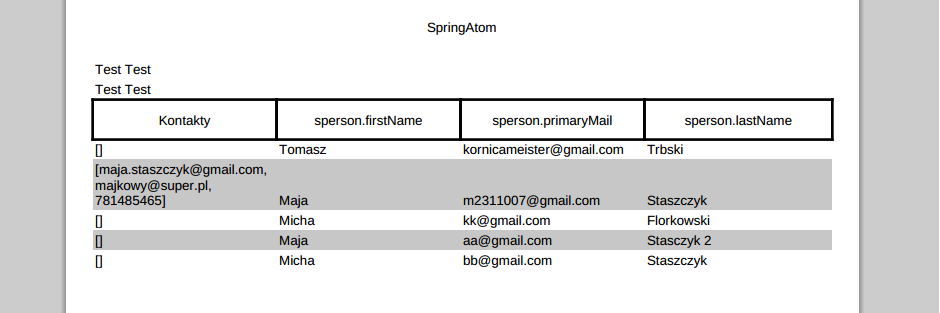
\includegraphics[width=1.0\textwidth]{images/rbuilder_report}
		\caption[Gotowy raport utworzony przez komponent \textbf{RBuilder}]{
			Gotowy raport utworzony przez komponent \textbf{RBuilder}, źródło: opracowanie własne
		}
		\label{app:wizard_newReport_report}
	\end{figure}	
	
